% Activate the following line by filling in the right side. If for example the name of the root file is Main.tex, write
% "...root = Main.tex" if the chapter file is in the same directory, and "...root = ../Main.tex" if the chapter is in a subdirectory.
 
%!TEX root =  

\chapter{Design}
\label{design}

\minitoc

This chapter details the organization and interaction between the different program components and the rationale for their design. The implementation of the framework is directly dependent on the design presented here, but the design is independent of programming languages and tools used in implementation

The structure of the program follows the CBR agent model discussed in the paper by T{\o}ndel, Nyre and Bernsmed (2011)\footnote{\emph{Inger Anne T{\o}ndel \& {\AA}smund Ahlmann Nyre \& Karin Bernsmed}: "Learning Privacy Preferences", SINTEF ICT, 2011.}. Given the broad structure of the model, several details need to be fleshed out, including data structures for storing policies, databases, choosing actual algorithms, a user interface, and so forth. This chapter lays out the broad structure of the Privacy Advisor system. Implementation details are discussed in the next chapter. The Section~\ref{desOverview} provides an overview over core functionality, including algorithms as well as program flow. The remaining sections cover data storage and user interfaces.


\section{Core Functionality}\label{desOverview}
In implementing Privacy Advisor, a class structure is built around the CBR agent model discussed in T{\o}ndel and Nyre. Refinements which must be made include data structures for storing policies, databases, choosing actual algorithms, and so forth. This section describes how the design in broad terms. 


\begin{figure}[htbp]
\begin{center}
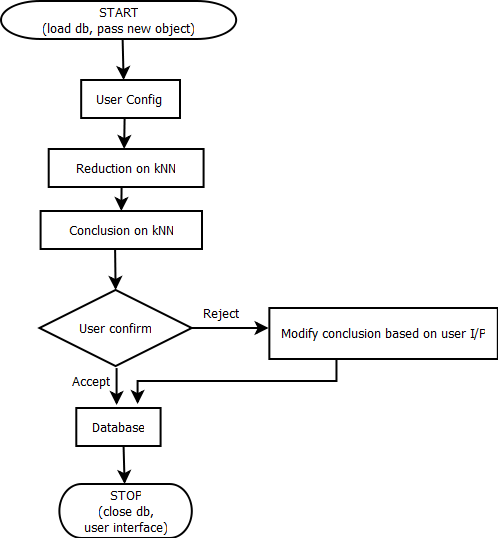
\includegraphics[width = 0.50 \textwidth ]{DesignReport/uml/flowchart.png}
\caption{Program Flow.}
\label{DesignFlowChart}
\end{center}
\end{figure}


\begin{figure}[htbp]
\begin{center}
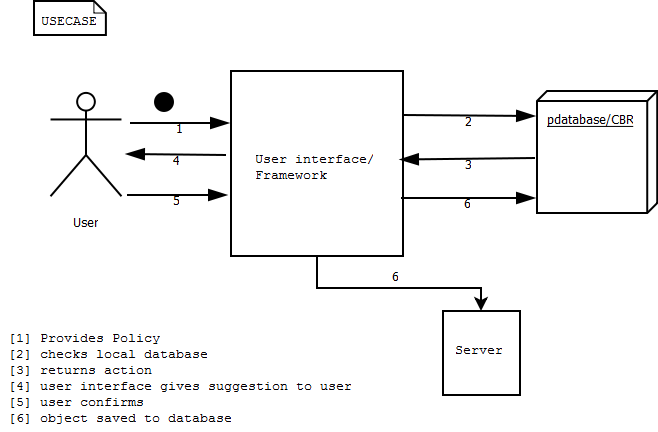
\includegraphics[width = \textwidth]{DesignReport/uml/Case.png}
\caption{System Overview.}
\label{SystemOverview}
\end{center}
\end{figure}

\subsection{Program Flow}
The discussion in this chapter focuses on the program flow for the command line version of Privacy Advisor. The GUI version follows a similar, but slightly more complex flow. The discussion is based on the standard flow where a database is already compiled and the user 

Figures~\ref{DesignFlowChart} and \ref{SystemOverview} seek to provide a broad overview of the structure of the Privacy Advisor system. The program flow is given by Figure~\ref{DesignFlowChart}: a policy object is passed to the CBR system from the user, either through the CLI or GUI. The CBR does a lookup on similar cases in the local database and computes an initial recommendation based on the similar cases retrieved. 

If the confidence in this recommendation is above a given threshold, it provides the user with the advice and the background for the advice through the user interface. If the confidence is not sufficient, the system will query the community system for an advice, which then is combined with the initial recommendation for a final advice which is presented to the user. The user can then provide feedback on the proposed solution, choosing to accept or reject it. The case along with the modified solution is subsequently retained in the knowledge base.

\begin{figure}[htbp]
\begin{center}
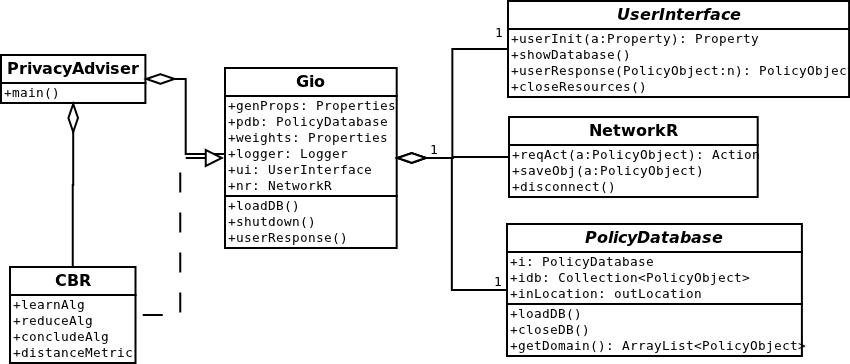
\includegraphics[width = \textwidth]{DesignReport/uml/main_2.png}
\caption{Privacy Advisor system overview.}
\label{overviewFig}
\end{center}
\end{figure}


\subsection{Top Level Design}
The program follows the general Case Based Reasoning cycle by first loading and initializing all components, then applying the relevent 'retreive' and 'reuse' algorithms, providing the suggestion to the user and waiting for a response during the 'revise' phase, and finally, saving the new case to the database and improving the distance metrics during the 'retain' phase (all seen in the figure \ref{DesignFlowChart}).
This is implemented in several different types of classes. The PrivacyAdviser 'main' class directs the flow from initialization and loading the the local history to the full CBR cycle, and if modified, allows the cycle to be reinitiated. The 'Gio' class handles the specifics of initializing most of the variables and classes - including the PolicyDatabase, which is then called to load according to its own design. CBR contains the control flow of the CBR cycle itself, creating and running the algorithms at the appropriate times, interacting through 'Gio' to access the local and remote database, as well as any necessary variables. The seperation of the CBR class from the 'main' class allows for an alternative machine learning algorithm, if one can be implemented such that it uses the provided interface. The 'Gio' class also holds the only reference to the user interface, which must provide a call for modifying the start-up variables, an interaction with the user, and the ability to display the database. Unless the user interface ('UserIO') is also the 'main' class, the program flow is strictly dictated and of finite length.

Figure \ref{overviewFig} is a UML class diagram of the high level structure of the program. When called, \texttt{PrivacyAdvisor} will call \texttt{Gio} to parse command line arguments. 


\subsubsection{CBR} 
Input from the UI is passed on to the CBR framework. CBR in turn references three other key modules, a \emph{reduction} algorithm, a \emph{conclusion} algorithm, and finally, a \emph{learning} algorithm. An overview of the CBR system is given in Figure~\ref{cbr_fig}.

\begin{figure}[h!]
\begin{center}
\includegraphics[width = \textwidth]{DesignReport/uml/CBR.png}
\caption{CBR System.}
\label{cbr_fig}
\end{center}
\end{figure}

The reduction algorithm, which in CBR terminology often is referred to as the \emph{retrieval algorithm} searches the database to find the most similar cases to the new case presented. The standard reduction algorithm is k Nearest Neighbors (kNN). kNN is discussed in section~\ref{kNN}. The conclusion algorithm looks at the set of cases returned by the reduction, and decides on the most appropriate action for the novel case. It also returns a measure of confidence in the conclusion reached. In CBR terms, this corresponds to the \emph{revise} phase.

Finally, a learning algorithm allows for automatically tuning the parameters used for distance calculations. The rationale for this augmenting of the classical CBR framework is the high dimensionality of the data. Without a manual learning approach it is hard to tell the system which fields in a policy is important in determining the similarity between two policies. Learning algorithms are discussed further in section~\ref{learnAlgos}.


\section{Data Objects and Storage}

The Privacy Advisor framework uses two key types of data storage that needs to be specified, one for storing the privacy policies and one for the databases holding the policies.

\subsection{P3P Policy Objects}\label{p3pPolObj}\index{P3P}
A P3P Policy Object consists of an \texttt{Action}, a \texttt{Context} and a list of different \texttt{Case} objects. The action object consists of the result from the comparison algorithm, stating if the policy is accepted as a good match, the reasons for this statement and with how much confidence this statement is correct. An overview of the Policy Object is given in Figure~\ref{po_fig}.

The context objects holds most of the objects context, that is what domain the policy belongs to as well as when it was created, last accessed and when it will expire. The list of cases contains one case for each datatype within the policy. A datatype is what kind of information is collected, for example name or date of birth. Each case contains what the purpose for this information is, who are the recipients and the retention for this information. Each datatype has its own case as it simplified the comparison algorithm.

The last thing a policy object contains is a hashmap of the entity data. This is the data that is included at the beginning of every policy document and contains information about the company in question.

\begin{figure}[htbp]
\begin{center}
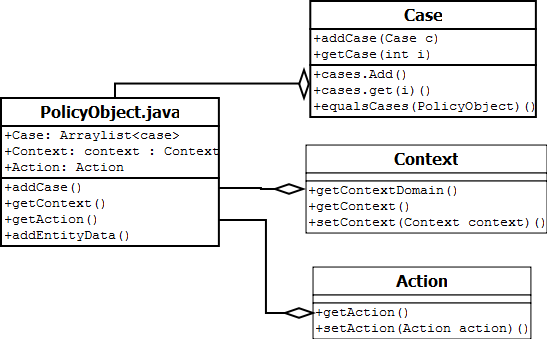
\includegraphics[width = \textwidth]{DesignReport/uml/po.png}
\caption{Policy Object.}
\label{po_fig}
\end{center}
\end{figure}

\subsection{P3P Policy Database}
The local case history, maintained in a local database, is stored via a concrete class implementing 'PolicyDatabase'. This abstract class details the required methods for a local policy database: a singleton constructor for the database object; a call to load the database once constructed, from disk; a method adding a single policy to the database; a method returning a Java iterator over the stored PolicyObjects, and a call to return all policies from a given domain. An overview of the Policy Database is given in Figure~\ref{pd_fig}.

In order to ensure consistency, the local policy database enforces singletonness. The database object itself is constructed without the actual history, requiring a seperate parameter-less 'loadDB' call on it to load policies from disk to the class, if necessary.
During the CBR cycle, it becomes necessary to check past cases for relevancy during the 'retrieve' phase. This is accomplished by using the standard java Iterator return by \texttt{getiterator()}.
Finally, the CBR cycle concludes by saving the new case (using 'addpolicy(newpolicy)'), and closing the database using 'closeDB()' (which is when the cases would be saved to disk).



\begin{figure}[htbp]
\begin{center}
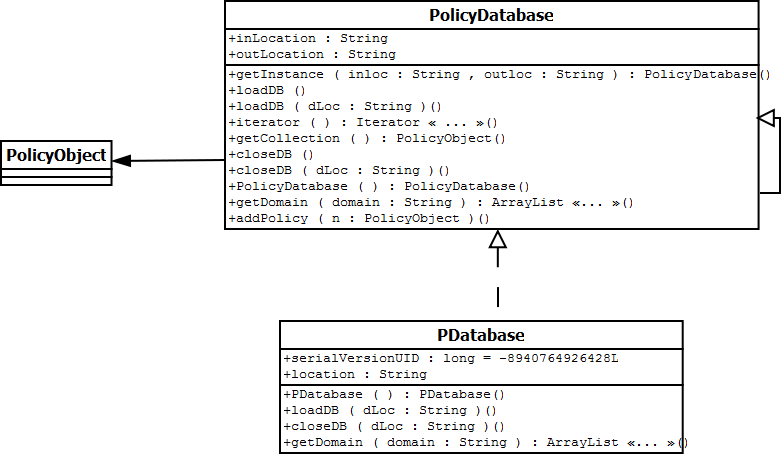
\includegraphics[width = \textwidth]{DesignReport/uml/pd.png}
\caption{Policy Database.}
\label{pd_fig}
\end{center}
\end{figure}



\subsection{Community Server}\index{Datastorage}\index{Datastorage!Community database} %%TODO needs rewrite- focuse here is on design not implementation. mention query should be server-side
The community knowledge repository is implemented using a public CouchDB (no-SQL server), which is accessed using standard Java to JSON java libraries. The client program (end-user java application) communicates with the server at two points- when the application has insufficient knowledge, or confidence in its knowledge, to make a suggestion as to the acceptance of a new P3P policy; and after the user has confirmed or overridden the policy.

In the first instance, the new policy under consideration is converted to JSON using GSON (the Google Json libraries), and transmitted to the database, which parses the new policy and replies with a JSON encoded suggested Action.

In the second instance, the final policy (including the action taken on it) is sent to the CouchDB server, and the server proceeds to store the object.
On the database end, there are two essential interfaces (beyond any standard initialization and shutdown procedures). As seem above, these two interfaces are the suggestion provider, which includes a query to find the most similar policies and actions on them by the community, and a interface to simply save the new policy to the appropriate database.
The database is easily replaceable, requiring only the construction of a new class implementing 'NetworkR', the abstract class detailing the methods called by the PrivacyAdvisor framework. The selection between available 'NetworkR' implementations in made by setting the 'NetworkRType' configuration variable during initialization to the full classname.
	




\section{User Interfaces}
Privacy Advisor can be run using either a command line interface (CLI) or a graphical user interface (GUI). Both the CLI and the GUI are built on top of a "General Input/Output'' module, GIO. GIO creates the database objects and issues the proper commands to the CBR framework based on user input. The GIO class is shown in Figure~\ref{GUI_interface}. 


\subsection{Graphical User Interface} 
The Graphical User Interface is used to get a graphical overview over the database, as well as change configurations and run the framework itself. The database is shown in a tree structure so that one can easily click through it and have a look at it. Configurations, reloading of the database and running the program can all be done from the PrivacyAdvisor drop-down menu.

After the program is run, a view of the new policy can be seen for reference in another view, also in a tree structure.

\begin{figure}[htbp]
\begin{center}
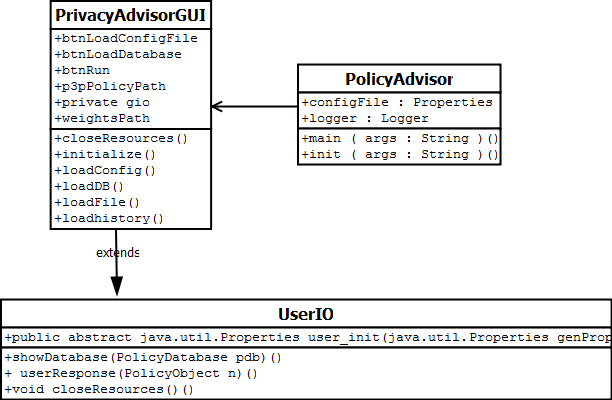
\includegraphics[width = \textwidth]{DesignReport/uml/policyadvisorgui}
\caption{GUI interfaces.}
\label{GUI_interface}
\end{center}
\end{figure}

\subsection{Weights and Configuration Files}
As an addition to passing command line arguments, GIO also reads a text based configuration file containing CBR and database settings. The configuration files are detailed in the User Documentation in the Appendix. 